\section{Design}\label{sec: Design}
In this section the design and decisions that where made to achieve the laboratory are discussed.

\subsection{Part I - Behavioral Modeling of a Seven-Segment Display}\label{subsec: Behavioral Modeling of a Seven-Segment Display}
Verilog is used to describe a decoder that shall control a seven-segment display with two switches and one button. The given task is as followed:
\\
\\
In this part, you will simulate a pattern decoder using the buttons, switches, and a single seven-segment display.
Using switches, SW0 and SW1 as the pattern input, write a Verilog program that takes the binary input
combinations of the switches and displays the decimal value of the binary switch combination on the seven-segment
display. Table 1 shows the switch combinations with the expected output value on the seven-segment
display.

\begin{figure}[htbp]
	\centering
	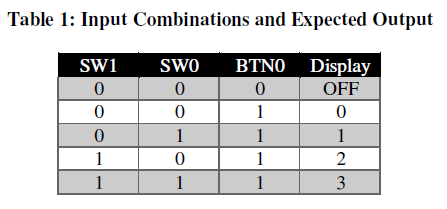
\includegraphics[width=0.6\textwidth]{01_images/Vivado_lab2_part1_table1.png}
	%\caption{Schematic directional coupler \cite{Vizmuller1995}}
	\label{fig: Vivado_lab2_part1_table1}
\end{figure}

As software package to implement the decoder in Verilog Vivado 2017.2 is used. 

\subsection{Part II - Hardware Implementation \& Modular Design}\label{subsec: Hardware Implementation Modular Design}
For the second part a hierarchical design is achieved including the implementation and generation of a bit stream to use hardware or more specific the PYNQ development board. Therfore the folowing task is given:
\\
\\
In this part, you will modify your code from Part I. Instead of only using one button and one switch, you will
design your Verilog code to display on four seven-segment displays by pressing the four buttons on the PYNQ
board. Each seven-segment display will correspond to one button (i.e., BTN0 lights up the right-most seven-segment
display and BTN1 will light up the adjacent seven-segment display and so on). Make sure that when a
button is released, the corresponding seven-segment display turns OFF. Only one seven-segment display should
be on at any given time.
\\
\\
To realize the constrained file the PYNQ reference manual was used to allocate the right pins for the switches and buttons, figure \ref{fig: PYNQ_BasicIO} shows the basic I/O pins assignment of the PYNQ development board.
\begin{figure}[H]
	\centering
	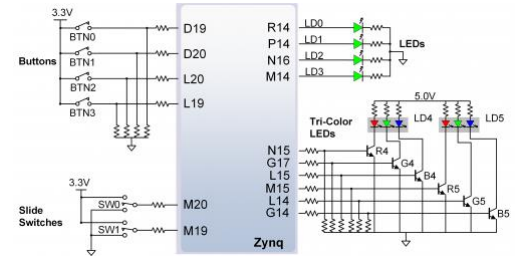
\includegraphics[width=0.6\textwidth]{01_images/PYNQ_BasicIO.png}
	\caption{Schematic PYNQ Basic I/O. \cite{PYNG_RM}}
	\label{fig: PYNQ_BasicIO}
\end{figure}
The one of solution to part II is two concatenated case statements. The first case is used to check for the button press and the second to switch the seven-segment display to show the number as defined by the two switches SW0 and SW1. The used code is listed in the following three listening \ref{lst: decoder part II}, \ref{lst: decoder top level part II}, and \ref{lst: decoder Constrains part II}.

\subsection{Part III - Laboratory Exercise}\label{subsec: Part III - Laboratory Exercise}
The third part of the lab combines part one and part two to a final design that uses a modified decoder version of part two and a clock divider to print out the words, PYNQ, FPGA, IS, and COOL with the seven-segment display. The clock divider is used to slow down the 125 MHz clock to 125 Hz, the relation ship of clock divider an decoder is shown in figure \ref{fig: Vivado_lab2_part3_block_diagram}. Switches SW0 and SW1 defines which word will be shown on the displays if the button BTN0 is pressed, as shown in figure \ref{fig: Vivado_lab2_part3_InAndOutTable}. The task is described as followed in the lab report: \\   
\\
In this part, you will create a time multiplexed seven-segment decoder using the block diagram shown in Figure
8 as a guide. You will need to create a multiplexer in order to display more than one seven-segment
simultaneously. Design the multiplexer to enable each digit for 8ms, or a 125Hz refresh rate. Remember, these
Pmods have a shared digit select pin. Most multi-digit displays would have a separate digit select pin for each
digit. Table 3 shows the required outputs for the required input combinations.

\begin{figure}[H]
	\centering
	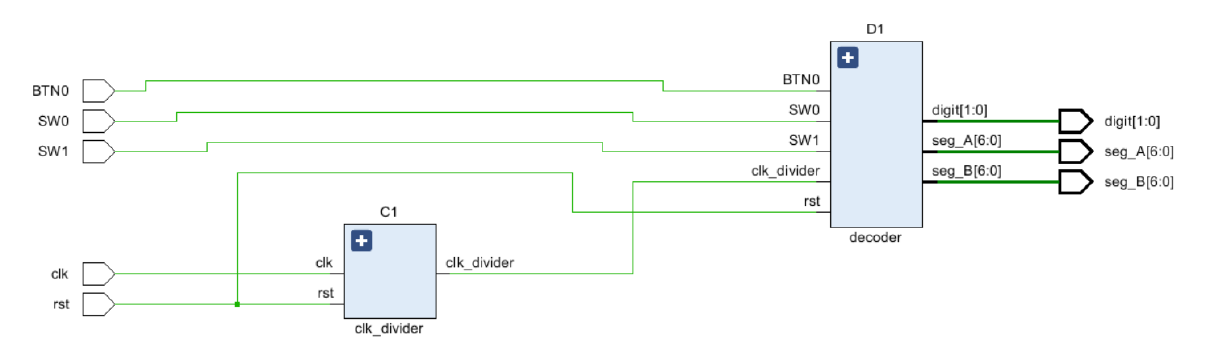
\includegraphics[width=1.0\textwidth]{01_images/Vivado_lab2_part3_block_diagram.PNG}
	\caption{Part III block diagram. \cite{PYNG_RM}}
	\label{fig: Vivado_lab2_part3_block_diagram}
\end{figure}
\begin{figure}[H]
	\centering
	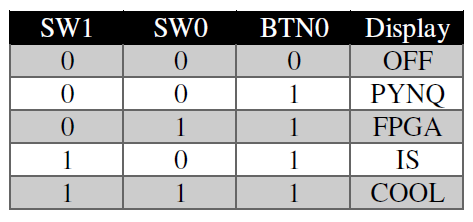
\includegraphics[width=0.5\textwidth]{01_images/Vivado_lab2_part3_InAndOutTable.PNG}
	\caption{Part III inputs and outputs. \cite{PYNG_RM}}
	\label{fig: Vivado_lab2_part3_InAndOutTable}
\end{figure}

The clock divider is realized with a counter that counts up until the divider ratio is reached of 500,000 as calculated with equation \ref{eq: div ratio}.

\begin{equation} \label{eq: div ratio}
	Divider\ ratio = \frac{f_1}{f_2 * 2} = \frac{125 MHz}{125 Hz * 2} = 500,000
\end{equation}
Therefore, a clk\_temp register is used to count up until the counter value equal or great than 500,000 is reached. In the top module the divided clk\_out of the clk\_divider is wired into the decoder. The reason is why the clock needs to be divided at the first placed is that a two fast clock would prevent the viability of the seven-segment displays. 
The decoder is time multiplexed because each seven-segment display has a common carriage line to display ever a number on display A or display B. Therefor, a time multiplexer was written which is clock depended that each display one after another.
The time multiplexer is realized with a case statement and a two bit value that iterates trough and each case displays one character of a word. 
\\ 
\\
Further improvements that would increase the code quality and re-usability of the  modules would be to change the clk\_divider module that the divider ratio is given as input to the clock divider. 
